% **************************************************************************************************************
% A Classic Thesis Style
% An Homage to The Elements of Typographic Style
%
% Copyright (C) 2010 André Miede http://www.miede.de
%
% If you like the style then I would appreciate a postcard. My address
% can be found in the file ClassicThesis.pdf. A collection of the
% postcards I received so far is available online at
% http://postcards.miede.de
%
% License:
% This program is free software; you can redistribute it and/or modify
% it under the terms of the GNU General Public License as published by
% the Free Software Foundation; either version 2 of the License, or
% (at your option) any later version.
%
% This program is distributed in the hope that it will be useful,
% but WITHOUT ANY WARRANTY; without even the implied warranty of
% MERCHANTABILITY or FITNESS FOR A PARTICULAR PURPOSE.  See the
% GNU General Public License for more details.
%
% You should have received a copy of the GNU General Public License
% along with this program; see the file COPYING.  If not, write to
% the Free Software Foundation, Inc., 59 Temple Place - Suite 330,
% Boston, MA 02111-1307, USA.
%
% **************************************************************************************************************
% Note:
%    * You must not use "u etc. in strings/commands that will be spaced out (use \"u or real umlauts instead)
%    * New enumeration (small caps): \begin{aenumerate} \end{aenumerate}
%    * For margin notes: \graffito{}
%    * Do not use bold fonts in this style, it is designed around them
%    * Use tables as in the examples
%    * See classicthesis-ldpkg.sty for useful commands
% **************************************************************************************************************
% To Do:
%		 * [high] Check this out: http://www.golatex.de/koma-script-warnung-in-verbindung-mit-listings-package-t2058.html
%    * [medium] mathbb in section-titles/chapter-titles => disappears somehow in headlines!!!
%    * [low] Calculate text block size for Libertine font
%    * [low] Think about processing a4paper, a5paper, 10pt, 11pt, 12pt etc. options for typearea layout
%            (store values in internal variables and handle by \AtEndOfPackage{\areaset...})
% **************************************************************************************************************
\documentclass[ oneside,openright,titlepage,fleqn,numbers=noenddot,headinclude,%1headlines,%
                11pt,a4paper,BCOR5mm,footinclude,cleardoublepage=empty,abstractoff % <--- obsolete, remove (todo)
                ]{scrreprt}

% ********************************************************************
% Development Stuff
% ********************************************************************
\listfiles
%\usepackage[l2tabu, orthodox, abort]{nag}
%\usepackage[warning, all]{onlyamsmath}
% ********************************************************************
% Re-usable information
% ********************************************************************
\usepackage[utf8x]{inputenc}
\newcommand{\myTitle}{Optimizing Operating System Imaging in University Deployments \xspace}
\newcommand{\myDegree}{Masters Thesis\xspace}
\newcommand{\myName}{Alexandru Juncu\xspace}
\newcommand{\myProf}{Conf. Dr. Ing. Răzvan Rughiniș\xspace}
\newcommand{\myOtherProf}{Ș.L. Dr. Ing. Răzvan Deaconescu\xspace}
%\newcommand{\mySupervisor}{Put name here\xspace}
\newcommand{\myFaculty}{Automatic Control and Computer Science Faculty\xspace}
\newcommand{\myDepartment}{Computer Science and Engineering Department\xspace}
\newcommand{\myUni}{\protect{University \emph{Politehnica} of Bucharest}\xspace}
\newcommand{\myLocation}{Bucharest\xspace}
\newcommand{\myTime}{July 2013\xspace}
\newcommand{\myVersion}{Version 1.0\xspace}


%*******************************************************
% Packages with options that might require adjustments
%*******************************************************
\usepackage[american]{babel}
\usepackage[square,numbers]{natbib}
\usepackage[fleqn]{amsmath} % math environments and more by the AMS

%*******************************************************
\usepackage{classicthesis-ldpkg} % [backref]
%*******************************************************
% Options for classicthesis.sty:
% tocaligned eulerchapternumbers rafting linedheaders listsseparated
% subfig nochapters beramono eulermath parts minionpro pdfspacing
% listings dottedtoc minionprospacing manychapters
\usepackage[eulerchapternumbers,listings,listsseparated,%pdfspacing,%listings,
						subfig,beramono,eulermath,parts]{classicthesis}

%*******************************************************
% Some font experiments
%*******************************************************
%\usepackage[osf]{libertine}
%\usepackage{hfoldsty}
%\usepackage[light,condensed,math]{iwona}
%\renewcommand{\sfdefault}{iwona}
%\usepackage{lmodern} % <-- no osf support :-(
%\usepackage[urw-garamond]{mathdesign} <-- no osf support :-(

%*******************************************************
% Fine-tuning for the text area
%*******************************************************
%\linespread{1.05} % a bit more for Palatino
%\areaset[5mm]{312pt}{761pt} % 686 (factor 2.2) + 33 head + 42 head \the\footskip
%\setlength{\marginparwidth}{7em}%
%\setlength{\marginparsep}{2em}%

%*******************************************************
% hack to use citations in float environments
% will be fixed with caption package version 3.2
%*******************************************************

%%%%%bug
\usepackage{makerobust}
\makeatletter
\MakeRobustCommand\caption@xref
\makeatother

%*******************************************************
%\usepackage[section,below]{placeins} <--- not everybody wants this
%\usepackage[all]{hypcap} <--- does not work with MiKTeX 2.6
% ********************************************************************
% Language/strings for backrefs (change here, thanks, Lorenzo)
%*******************************************************
%\renewcommand{\backrefnotcitedstring}{\relax}%(Not cited.)
%\renewcommand{\backrefcitedsinglestring}[1]{(Citato a pagina~#1.)}
%\renewcommand{\backrefcitedmultistring}[1]{(Citato alle pagine~#1.)}
%\renewcommand{\backreftwosep}{ e~}
%\renewcommand{\backreflastsep}{ e~}
% ********************************************************************
% Setup and Finetuning
%*******************************************************
\newlength{\abcd} % for ab..z string length calculation
\newcommand{\myfloatalign}{\centering} % how all the floats will be aligned
\setlength{\extrarowheight}{3pt} % increase table row height
% ********************************************************************
% Captions look and feel
%*******************************************************
\captionsetup{format=hang,font=small}
% ********************************************************************
% Listings setup
% ********************************************************************
%\lstset{emph={trueIndex,root},emphstyle=\color{BlueViolet}}%\underbar} % for special keywords
% ********************************************************************
\lstset{language=[LaTeX]Tex,%C++,
    keywordstyle=\color{RoyalBlue},%\bfseries,
    basicstyle=\small\ttfamily,
    %identifierstyle=\color{NavyBlue},
    commentstyle=\color{Green}\ttfamily,
    stringstyle=\rmfamily,
    numbers=none,%left,%
    numberstyle=\scriptsize,%\tiny
    stepnumber=5,
    numbersep=8pt,
    showstringspaces=false,
    breaklines=true,
    frameround=ftff,
    frame=single,
    belowcaptionskip=.75\baselineskip,
    numberbychapter=false
    %frame=L
}

% ********************************************************************
% Where to look for graphics
%*******************************************************
%\graphicspath{{gfx/}{misc/}} % considered harmful according to l2tabu
% ********************************************************************
% Hyperreferences
%*******************************************************
\hypersetup{%
    colorlinks=true, linktocpage=true, pdfstartpage=3, pdfstartview=FitV,%
    % uncomment the following line if you want to have black links (e.g., for printing)
    %colorlinks=false, linktocpage=false, pdfborder={0 0 0}, pdfstartpage=3, pdfstartview=FitV,%
    breaklinks=true, pdfpagemode=UseNone, pageanchor=true, pdfpagemode=UseOutlines,%
    plainpages=false, bookmarksnumbered, bookmarksopen=true, bookmarksopenlevel=1,%
    hypertexnames=true, pdfhighlight=/O,%hyperfootnotes=true,%nesting=true,%frenchlinks,%
    urlcolor=webbrown, linkcolor=RoyalBlue, citecolor=webgreen, %pagecolor=RoyalBlue,%
    %urlcolor=Black, linkcolor=Black, citecolor=Black, %pagecolor=Black,%
    pdftitle={\myTitle},%
    pdfauthor={\textcopyright\ \myName, \myUni, \myFaculty},%
    pdfsubject={},%
    pdfkeywords={},%
    pdfcreator={pdfLaTeX},%
    pdfproducer={LaTeX with hyperref and classicthesis}%
}

%********************************************************************
% Hyphenation
%*******************************************************
%\hyphenation{put special hyphenation here}
% ********************************************************************
% GO!GO!GO! MOVE IT!
%*******************************************************
\begin{document}
\frenchspacing
\raggedbottom
\selectlanguage{american} % american ngerman
%\renewcommand*{\bibname}{new name}
%\setbibpreamble{}
\pagenumbering{roman}
\pagestyle{plain}
%********************************************************************
% Frontmatter
%*******************************************************
%%*******************************************************
% Little Dirty Titlepage
%*******************************************************
\thispagestyle{empty}
%\pdfbookmark[1]{Titel}{title}
%*******************************************************
\begin{center}
    \spacedlowsmallcaps{\myName} \\ \medskip

    \begingroup
        \color{Maroon}\spacedallcaps{\myTitle}
    \endgroup
\end{center}

%*******************************************************
% Titlepage
%*******************************************************
\begin{titlepage}
  % if you want the titlepage to be centered, uncomment and fine-tune the line below (KOMA classes environment)
  \begin{addmargin}[-1cm]{-3cm}
    \begin{center}
        \large

        \hfill

        \vfill

        \begingroup
            \color{Maroon}\spacedallcaps{\myTitle} \\ \bigskip
        \endgroup

        \spacedlowsmallcaps{\myName}

        \vfill

        
\includegraphics[width=6cm]{gfx/cs} \\ \medskip

        \myDegree \\ \medskip
        \myDepartment \\
        \myFaculty \\
        \myUni \\ \bigskip

        \myTime

        \vfill

    \end{center}
  \end{addmargin}
\end{titlepage}

\thispagestyle{empty}

\hfill

\vfill

\noindent\myName: \textit{\myTitle,} \myDegree, \textcopyright\ \myTime

\bigskip

\noindent\spacedlowsmallcaps{Supervisors}: \\
\myProf \\
%\myOtherProf %\\
%\mySupervisor

\medskip

\noindent\spacedlowsmallcaps{Location}: \\
\myLocation

\medskip

\noindent\spacedlowsmallcaps{Time Frame}: \\
\myTime

%\cleardoublepage%*******************************************************
% Dedication
%*******************************************************
\thispagestyle{empty}
%\phantomsection
\refstepcounter{dummy}
\pdfbookmark[1]{Dedication}{Dedication}

\vspace*{3cm}

\begin{center}
    \emph{Ohana} means family. \\
    Family means nobody gets left behind, or forgotten. \\ \medskip
    --- Lilo \& Stitch
\end{center}

\medskip

\begin{center}
    Dedicated to the loving memory of Rudolf Miede. \\ \smallskip
    1939\,--\,2005
\end{center}

\cleardoublepage%*******************************************************
% Abstract
%*******************************************************
%\renewcommand{\abstractname}{Abstract}
\pdfbookmark[1]{Abstract}{Abstract}
\begingroup
\let\clearpage\relax
\let\cleardoublepage\relax
\let\cleardoublepage\relax

\chapter*{Abstract}
This thesis presents an advanced imaging solution for Operating System
Multiplication over the network based on UDP Cast with a suite of added
software. It presents the idea for a centralized archiving system and
distribution of the images over the network along with the deployment
of the solution.

The fist chapters present the features of UDP Cast, an open source project
for multicast transmission of data, along with the shortcomings of
UDP Cast.

The proposed project in the thesis focuses on implementing a system that
fixes the discovered problems. The idea presented is an architecture with
an Imaging Client and an Imaging Server.

The last chapters present the implementation of the Client and the Server,
ending with the evaluation on the model.



\endgroup

\vfill

%\cleardoublepage%*******************************************************
% Publications
%*******************************************************
\pdfbookmark[1]{Publications}{publications}
\chapter*{Publications}
Some ideas and figures have appeared previously in the following publications:

\bigskip

\noindent Put your publications from the thesis here.
%\cleardoublepage%*******************************************************
% Acknowledgments
%*******************************************************
\pdfbookmark[1]{Acknowledgments}{acknowledgments}

\begin{flushright}{\slshape
    We have seen that computer programming is an art, \\
    because it applies accumulated knowledge to the world, \\
    because it requires skill and ingenuity, and especially \\
    because it produces objects of beauty.} \\ \medskip
    --- \defcitealias{knuth:1974}{Donald E. Knuth}\citetalias{knuth:1974} \citep{knuth:1974}
\end{flushright}



\bigskip

\begingroup
\let\clearpage\relax
\let\cleardoublepage\relax
\let\cleardoublepage\relax
\chapter*{Acknowledgments}
Put your acknowledgments here.

Many thanks to everybody who already sent me a postcard!

Regarding the typography and other help, many thanks go to Marco 
Kuhlmann, Philipp Lehman, Lothar Schlesier, Jim Young, Lorenzo 
Pantieri and Enrico Gregorio\footnote{Members of GuIT (Gruppo 
Italiano Utilizzatori di \TeX\ e \LaTeX )}, J\"org Sommer, 
Joachim K\"ostler, Daniel Gottschlag, Denis Aydin, Paride 
Legovini, Steffen Prochnow, Nicolas Repp, Hinrich Harms, 
and the whole \LaTeX-community for support, ideas and some great software.

\endgroup




\pagestyle{scrheadings}
\cleardoublepage%*******************************************************
% Table of Contents
%*******************************************************
%\phantomsection
\refstepcounter{dummy}
\pdfbookmark[1]{\contentsname}{tableofcontents}
\setcounter{tocdepth}{2} % <-- 2 includes up to subsections in the ToC
\setcounter{secnumdepth}{3} % <-- 3 numbers up to subsubsections
\manualmark
\markboth{\spacedlowsmallcaps{\contentsname}}{\spacedlowsmallcaps{\contentsname}}
\tableofcontents 
\automark[section]{chapter}
\renewcommand{\chaptermark}[1]{\markboth{\spacedlowsmallcaps{#1}}{\spacedlowsmallcaps{#1}}}
\renewcommand{\sectionmark}[1]{\markright{\thesection\enspace\spacedlowsmallcaps{#1}}}%*******************************************************
% List of Figures and of the Tables
%*******************************************************
\clearpage

\begingroup
    \let\clearpage\relax
    \let\cleardoublepage\relax
    \let\cleardoublepage\relax
    %*******************************************************
    % List of Figures
    %*******************************************************    
    %\phantomsection
    \refstepcounter{dummy}
    %\addcontentsline{toc}{chapter}{\listfigurename}
    \pdfbookmark[1]{\listfigurename}{lof}
    \listoffigures

    \vspace*{8ex}

    %*******************************************************
    % List of Tables
    %*******************************************************
    %\phantomsection
    \refstepcounter{dummy}
    %\addcontentsline{toc}{chapter}{\listtablename}
    \pdfbookmark[1]{\listtablename}{lot}
    \listoftables

    \vspace*{8ex}
%   \newpage

    %*******************************************************
    % List of Listings
    %*******************************************************      
    %\phantomsection
    \refstepcounter{dummy}
    %\addcontentsline{toc}{chapter}{\lstlistlistingname}
    \pdfbookmark[1]{\lstlistlistingname}{lol}
    \lstlistoflistings

    \vspace*{8ex}

    %*******************************************************
    % Acronyms
    %*******************************************************
    %\phantomsection
    \refstepcounter{dummy}
    \pdfbookmark[1]{Acronyms}{acronyms}
    \markboth{\spacedlowsmallcaps{Acronyms}}{\spacedlowsmallcaps{Acronyms}}
    \chapter*{Acronyms}
    \begin{acronym}[UML]
        \acro{API}{Application Programming Interface}
        \acro{UML}{Unified Modeling Language}
        \acro{OS}{Operating System}
        \acro{GUI}{Graphical User Interface}
	\acro{CLI}{Command Line Interface}
	\acro{IP}{Internet Protocol}
	\acro{UDP}{User Datagram Protocol}
	\acro{TCP}{Transmission Control Protocol}
	\acro{PXE}{Preboot Execution Environment}
	\acro{DHCP}{Dynamic Host Configuration Protocol}
	\acro{TFTP}{Trivial File Transfer Protocol}
	\acro{TTL}{Time To Live}
	\acro{GZIP}{GNU zip}
	\acro{LZOP}{Lempel-Ziv-Oberhumer compresion}
	\acro{PIM}{Protocol Independent Multicast}
	\acro{IGMP}{Internet Group Management Protocol}
	\acro{IANA}{Internet Assigned Numbers Authority}
	\acro{MBR}{Master Boot Record}
	\acro{GPL}{Generic Public License}
	\acro{LAN}{Local Area Network}
	\acro{NIC}{Network Interface Card}
	\acro{HDD}{Hard Disk Drive}
	\acro{NTP}{Network Time Protocol}
	\acro{AS}{Autonomous System}
	\acro{RPF}{Reverse Path Forwarding}
	\acro{BIOS}{Basic Input Output System}

    \end{acronym}
\endgroup

\cleardoublepage

%********************************************************************
% Mainmatter
%*******************************************************
\pagenumbering{arabic}
% use \cleardoublepage here to avoid problems with pdfbookmark
%\cleardoublepage\part{Some Kind of Manual}
% vim: set tw=78 sts=2 sw=2 ts=8 aw et ai:

\chapter{Introduction}\label{ch:intro} \bigskip


Modern educational institutions, like most institutions today, rely
heavily on the IT infrastructure to provide quality services for
students. The computer network for such institution needs to scale to
the same level as a large company campus network, the students being the
equivalent of production employees. The infrastructure needs to provided
the needed service for the students to efficiently accomplish their
goals of learning new information aided by the modern technology
available.


But there are some things that make schools or universities computer
setups different from an enterprise level company. While in a company
each employee has its workstation setup suited for his or her needs,
with the software required for his or her job role, computers in schools
and universities are build for massive identical deployments. For
example, each computer lab, of 10-20 computers, needs to be set up for a
specific course. A computer would be used for and hour or two by a
student, and then another student needs to use it, preferably, in the
same conditions as the previous student. While a setup for 10-20
computers with identical images could be done with some effort, this has
to be done with the idea in mind that the lifespan of the image would be
for about one semester, until another course needs the lab.

These kinds of conditions make IT administrators of educational
environments think in another way than the IT staff in a company. Things
need to be optimised so that the maximum efficiency could be obtained
with as little effort as possible, because the setup needs to scale to
tens of computer labs.

Higher education schools could also have needs for server rooms that
provide students places to run projects on. In research universities,
processing power is essentials for research professors and students to
run their experiments.


The following paper will present in more detail an university
environment with its current and future needs, as well as present
proposals for using current available technologies to better administer
the available equipment and to create opportunities for new features to
be available to students and teachers. It will focus on the current
needs and proposed enhancements specific to the \emph{Computer Science
and Engineering Department of the University POLITEHNICA of Bucharest},
but the information could be useful for departments of universities with
similar conditions.

\section{Current implementation and technologies used}

There are a few requirements that an administrator of a computer
laboratory room needs to take into consideration.

First of all, the computer's operating system needs to be prepared for
the activities that will be conducted in the room. This could impose the
operating system itself (for example, for a Linux class you will prefer
not to install Windows on it), or just the applications needed (for
example, for a programming class you need to install IDE software).


Once you have the requirement list, you start installing the system.
When dealing with a large number or workstations, preparing each station
by itself would take a huge effort and a large number of work hours.
This is where imaging software solutions come in. Software like
\emph{UDPCast}, Norton Ghost or FOG could provide scalable operating
system installation by using a single system image and multiplying it to
the rest of the systems either by a large mobile media storage or using
the existing local area network.

The multiplication of the image brings another need in a class: the need
that every student has the same environment to work in as the next one.
This is important because the teacher doesn't need to waste time to
debug something that works for one student but doesn't for another
thinking that it's because one workstation is different than the other.
And the student doesn't need to feel lucky or unlucky while he or she is
working on a task because on the colleague's workstation a certain
software is installed and on his or her workstation, that tool isn't.

Multiplying the same operating system image to all workstations solves
that issue, but only for the first group of students that use those
workstations. Laboratory rooms change groups of students maybe 10 times
a day. Each group should have the same conditions as the previous group
that used the workstations. This is where an operating system freezing
solution comes in. A freezing system would make each boot of an
operating system the same as the previous one by the removing or
reverting the changes made between two restarts.


One other consideration that needs to be considered in advance is the
need for special equipment in the laboratory. For example there are labs
where a tasks could ask one student to administer 3 stations that are
connected to each other by network. Due to limited physical resources,
such laboratories are hard to implement. This is where \emph{virtual
machines} could provide solutions. A single physical system could host
several virtual machines configured in any needed topology. Special
equipment such as routers could be emulated in virtual appliances rather
than be physically installed in the laboratory room.

\section{Limitations of current deployment}


Although current procedures for maintaining a deployment of a large
number of computer lab room have proven themselves useful in raising
efficiency of administration costs, they do, however, have some
drawbacks.

The imaging system, using UDPCast has the issue that is hard to
administer without a central control point. By design, UDPCast is a set
of programs that need to be activated individually, on each workstation.
This is usually done by using either a LiveCD or a LiveUSB stick that
contains the UDPCast mini Linux Distribution and having to go to each
workstation and booting it, configuring either the client or the server
and starting the imaging process manually on each machine.

This could be speeded up by having the image for the UDPCast (kernel and
initial RAM disk) stored on the harddrive of the physical machines, but
this is a chicken-before-egg problem because you have to first put that
image on each station. Booting the UDPCast image off the network using
PXE could be more efficient, but that is still limited by the fact that
you have to make every workstation boot off PXE and not local disk and
the fact that setting up a PXE server in the local network is a
challenge by itself.

Some fixes for problems regarding UDPCast have been presented in an
earlier related work \cite{paper:me}, proposing a centralized
architecture built around UDPCast. Although easier to manage, that
approach is also limited to problems related to \ac{PXE} and the need
for a communication channel between clients (the workstation) and a
server (the central control point).


The freezing system is good because it lowers the need for re-imaging a
large number of workstation a certain period of time, keeping the same
environment for all workstations in a room. The weakness of the freezing
system is also in its architecture.

The operating system is "froze" by using a freezing partition (it can
also be just a file on the partition) to store the modifications done to
the current session. The files of the base image are never modified, all
that is modified are the files on the freezing partition. But for the
files to exist on the freezing partition, they need to be copied from
the base partition. This introduces a large IO overhead. When accessing
large files in the operating system, they have to first be copied to the
freezing partition that introduces latency between access time and data
available time.


Virtual machines that could be copied to each workstation, having inside
the contained environment needed, could replace the need for having the
need to keep the same operating system image on all workstations. Each
workstation could have its own operating system and provide a
virtualization hypervisor to run a standard virtual machine. This would
make the freezing system useless and lower the need for system-wide
reimaging.

But because modern operating system have grown in requirements,
especially in hard disk space size needed, there is the problem of
deploying them across all workstations. There is also the limitations of
some older workstation that don't have the physical resources to
smoothly run fully functional virtual machines.

A special mention of a deployment need at UPB is the \emph{VMChecker}
infrastructure. Currently not connected to the laboratory
infrastructure, it's a set of servers used in automated homework
checking. The system uses virtual machines that provide an independent
environment of testing of student homework assignments. The virtual
machines used the automated system have ties to the ones used in student
classrooms.

\section{New technologies and procedure optimizations}


Technological innovations bring new opportunities for experimenting
towards improving workflow of administering the given environment. Such
innovations include new operating system features and new software ideas
but also hardware improvements for computer systems and advances in
protocols for the network that connects the computers together.


\emph{Virtualization} is one of the most fast growing market in computer
science and computer engineering. Processor producing companies,
software companies, application and kernel developers are investing
time, effort and money into providing better virtualization solutions.

Intel and AMD are already shipping all new processors with their new
hardware virtualization technologies (\emph{\ac{Intel VT}} and
\emph{\ac{AMD-V}}).
Other hardware component companies are investing in technologies for
assisting virtualization such as Pass-through component virtualization.

On the operating system side, system and kernel developers are improving
all virtualization solusions. While the open source community are
pushing projects like \emph{\ac{LXC}/OpenVZ}, \emph{\ac{Xen}} and
\emph{\ac{KVM}},
companies like VMware are investing in their own proprietary approaches.

These technologies are brought together and controlled by management
software that makes administration of a large number of virtual machines
and their foundation, the pool of physical machines, as easy and as
transparent to the user as possible. This idea has been introduced to
the world as the notion of \emph{Cloud computing} that puts emphasis on
better hardware resources utilization, easy provisioning and security
through backup and quick migration.

The push towards distributed systems is made possible because of the
advances of the processing power of each node and also the advances in
networking technologies that connect the nodes. Gigibit Ethernet is
becoming a standard for the \ac{LAN}. This makes not only transferring
large amounts of data over the network faster, but also with less
latency. This is what allows computers to act like terminals and have
the data not only on the local system, but over the network, either on a
nearby workstation or on a remote server.

But one of the most important new technology, and one of the main focus
of this thesis is the introduction of management tools that are both in
software and in hardware. This makes administration of a large network
scalable. Such a technology is Intel's  \emph{vPro}. This will be
discussed in more detail in later chapters.

\section{Purpose of this thesis}

This paper proposes an architecture to be used in deployments of large
computer deployments for educational purposes. The plan is to use a
distributed approach of processing and data storage using classroom
workstations as the nodes.

The workload of the nodes will be in the form of hypervisors for virtual
machines running on those physical systems. The network will be used for
distributing the virtual machines and keeping them synchronized to
provide an homogeneous environment for the users.

The virtual machines will be available as a pool of template machines,
each template made for a certain task (in this case, a specific
classroom environment).

The hypervisors will be Linux-basses machines using open source
technologies like Qemu-KVM, LXC and Xen. The software solutions will be
assisted by hardware virtualization technologies like Intel-VT.

The management of the hardware infrastructure will be done using the
remote management solutions provided by Intel vPro technology.

For the massive data transmission needed for imaging a cluster of
workstations, open source solutions such as UDPCast and rsync or SMB or
NFS are used.

The following chapters will provide a more in depth description of the
proposed optimizations.

The thesis will also provide a case study of how to use the proposed
infrastructure to be used for projects such as VMChecker that could be
made more efficient by scaling its physical resources. The case study
proposing provisioning unused physical machines from the computer
laboratories as clusters for VMChecker.

% vim: set tw=78 sts=2 sw=2 ts=8 aw et ai:

\chapter{Current deployment}\label{ch:current}
\bigskip

\section{UDPCast}


Setting up a computer means two things: getting the hardware (a normal
PC) and installing a modern Operating System on it to control that
hardware. This is a job that would take a normal person, with basic
computer operating skills, about one hour on average. However, the
normal approach does not scale to installing on 3 or more hosts that
need the exact same setup.


In office environments, Internet/Game Cafes and, most important, in
school laboratories where 15 to 20 computers with identical
configuration need to be set up, an imaging solution is needed.  This
means that the setup will be done on a single computer and then, the
entire disk on which the new operating system resides is copied
throughout the network onto the disks of the other uninstalled hosts.
This can save, for a number of 20 hosts, from 20 hours of work to only
two hours (about one hour for installing one system and another hour
for the copy of the disk(s) over the network).


To get a perfect mirroring, it is recommended that the hosts be
identical (same CPU, same Main board, same \ac{HDD}s, same network card).
If the systems differ in a slight way, it is up to the operating
system to try and adapt to new hardware and install the appropriate
drivers.  From the operating system’s point of view, it is like the
HDD was taken out of one computer and installed in another one.

\begin{figure}[h]
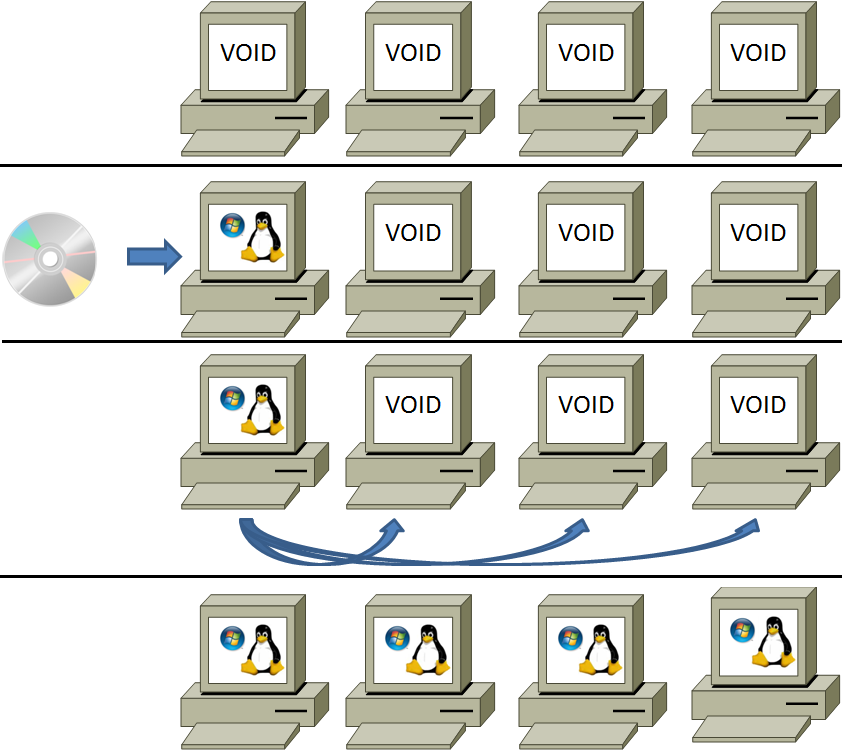
\includegraphics[width=10cm]{img/4comp}
\caption{Simple imaging operations}
\label{fig:4comp}
\end{figure}


To image a network of stations, there are some basic steps you need to take

\begin{enumerate}
\setcounter{enumi}{0}
\item Prepare all the hosts so they can power on. They can have empty
hard disks or hard disks with data that can be deleted.


\item Install one or more operating systems on one host.  This host will
be the seed host.  The operating system(s) can be personalized with
user accounts, installed programs, configured environments. Along with
the operating system(s), on the hard disk there will be the stage 1
boot loader in the \ac{MBR} and the upper stages of the boot loader on
other partitions. Separate partitions for personal data or backups can
be created


\item All the hosts must be able to boot in a pseudo-operating system
provided by the imaging software from a Live CD,  over the network via
PXE or from a local special partition so the working operating is not
modified during the imaging operation.


\item The contents of the seed’s hard disk are copied over the network
(usually using UDP over Multicast IP).  After the transfer is
complete, all hosts boot up normally.
\end{enumerate}



When using imaging systems, software licensing must be taken under
consideration.  The software that has per host or per CPU license has
to have a separate license code for each host.
There are two widely used software suits that provide system imaging:
Symatec Norton Ghost and UDP Cast. The first one is a professional
closed source enterprise software while the second one is an open
source project developed by a community.  Because of the flexibility
of open source projects, UDP cast, has been used in the development of
this imaging system solution and will be described in more detail.

UDP Cast is an open source project that offers a file transfer tool
that can send data simultaneously to many destinations on a \ac{LAN}, under
the \ac{GPL} 2.0 License. The program, along with its source code can be
downloaded from their site, at http://udpcast.linux.lu/.
The compiled projects, offers two executables:  udp-sender and
udp-receiver. By default, the two programs can be used to send input
from standard input on the sever side to all the clients which print
the received data to standard output.


On top of the two executables (udp-sender and udp-receiver) the UDP Cast
Project offers a Live CD (that can be found on their website) built to run
a wizard for the configuration for a sender or a receiver of a system
image. The iso file can be burned onto a CD or set up on a PXE network
boot.

The Live CD is a Linux Distribution based on Debian, stripped down to
occupy a small amount of memory and boot very fast. It must be booted on
all workstations that will participate in the imaging process (the seed
that is the sender and all the receivers)

After the kernel loads, it must load kernel modules (device drivers)
for the \ac{NIC} and the hard disk drives.


When the \ac{OS} has loaded the device driver, it can configure
network connectivity. This is done either by setting up a manual IP address
with a valid subnet mask or by use of \ac{DHCP} automatic configuration.
Obtaining an IP address is mandatory for the system to work because,
without an IP, the sender can't connect to the receivers.



After the device driver for the hard disks (PATA, SATA, SCSI) is loaded,
the user must chose what partition or device will be imaged. This has local
significance. On the seed host it will be the partition that will be sent over
the network and on the receivers it will be the partition on which the data
will be written. The name of the partitions are Linux formated. The user
can select a single primary or logical partition (ex. hda1, sda2, sdb5) or
an entire drive (hda, hdb, sda). The \ac{MBR} is found on the first 512bytes of
the physical drive.

It is recommended that the same option be selected on all devices.



A partition is usually has a very large data size and the transfer over the
network could be time consuming. For computers with good enough processing
power, compression can be used. UDP Cast offers two types of compression
\begin{itemize}
\item \ac{LZOP}
\item \ac{GZIP}
\end{itemize}

The use of compression can reduce the sent data by a factor of up to 50\%.


After all the configurations are made (they should be identical in most
conditions), the direction of the transfer must be specified on each host.
One workstation will be the sender and all the others will be the
receivers.


A proposed optimisation of using the UDPCast in laboratory environment
has been discussed in a previous thesis that I authored \cite{paper:me}.
It presents a centralized approach using a Python based client-server
architecture. While this creates a central node that stores a database
of operating system images, it cannot control the other nodes remotely.
This is a pull model where the administrator has to visit each node and
configure it to ask for an image from the server.

The centralized architecture has the big drawback of making the
administrator physically move between stations to complete the work.

Another problem with that approach is the fact that the client-server
protocol proposed is in a very early stage of development so it is not
an industry standard.

Some of these problems could be resolved given a proper remote
management system.

\section{Freezing script}

The freezing script has been developed by Mircea Bardac and Geroge
Milescu from the Computer Science Department at UPB. The central part of
it is the \ac{AUFS} filesystem that is used an intermediary layer for
the operating system's root file system. This script is made for Linux
distributions.

A normal boot of a Linux distribution has its root filesystem hierarchy
can be mounted from one or several partitions. Those mountpoints are
usually in read-write mode. With the exception of mountpoints such as
/proc and /dev that use the procfs and devfs filesystems, any \ac{IO}
results will results in changes on the physical partition.

The \ac{AUFS} mountpoints act as an extra layer in the IO operations
stack.The freezing script requires an extra partition reserved on the
hard drive (or a large file, like a swapfile). The \ac{IO} operations
will be done in the Linux \ac{VFS} are done as usual, but are
intercepted the \ac{AUFS} and the changes aren't pushed on the physical
device, but wrote in the special freezing partition.

While the system is running, the freezing partition is used in a
\ac{COW} mode: when files are needed from the root partition, they are
copied to the freezed partition and used from there. At a reboot, the
freezing partition changes are ignored and the files from the root
partition(s).

For Windows systems, a similar, enterprise and closed source product is
available: \emph{DeepFreeze}.

The architecture of the system gives an inherited flaw: the latency
caused by sometimes needing to double copy. If large files are involved,
the latency is visible to the user.


\begin{table}
\begin{tabular}{|p{4cm}|p{3cm}|p{3cm}|}
\hline
Action & Time on no-freezed syste & Time on freezed system \\
\hline
Write 1GB file from /dev/zero & 6.7s & 6.7s \\
\hline
Reading newly created file (1GB) & 1.4s & 1.5s \\
\hline
Reading file from root system (1GB) & 1.4s & 8.1s \\
\hline
\end{tabular}
\caption{Latency when using freezing system}
\label{table:aufs_latency}
\end{table}

As seen in table \ref{table:aufs_latency}, writing or reading new files
has no impact on IO times because the operations do a single write (one
to the root partition directly one to the freezing partition, directly).
But when you access a file that exists on the root partition, it first
needs to copy the file from the root partition to the freeze partition,
and that could take as much as 5 times more time.

A new approach for a freezing system with support in the Linux kernel
has been discussed in another thesis \cite{paper:freezing}.

\section{Virtual machines}


Virtual machines have become essential in computer laboratory rooms.
They provide easy to setup and deploy environments.

A thorough presentation of what virtualization is, what are the current
available technologies and what is their role in education is covered by
Huber et al. \cite{paper:virtualization}. The term virtualization refers
to any abstraction of a physical system and its resources from
asoftware. The virtualization can be for an application, a process or an
entire operating system. The main purpose of a virtualized environment
is to provide a layer of security by containing the guest system from
interacting with the main hardware or the resources from another guest.

There are a number of types of virtualization, each with its own
approach and its use-case.

\emph{Virtual memory} is one of the first ways of virtualizing hardware.
Rather than each process of an operating system having access to the
main physical memory, it has access only to its own virtual memory This
secures one process from all other processes on the system and gives
each process the same amount of memory, regardless of the actual
physical memory, offering portability of the process code. The
operations on the virtual memory is supervised by the operating system
and uses the \emph{ MMU (Memory Management Unit)} that needs hardware
support.

\emph{Emulators} hide the real hardware from a guest by rewriting every
hardware operationin software. A virtualized process or operating system
would run inside a process in the host’s operating system. Any
architecture can be emulated in software but at a high loss of
performance. QEMU, Dynamips or DosBox are examples of emulators.

\emph{Paravirtualization} uses a hypervisor to trap operations from a
guest machine and makes decisions on weather to resolve them by itself
or to send them to the actual hardware to be resolved. Xen is a
paravirtualization solution.

\emph{Hardware-assisted virtualization} is a form of full
virtualization, in which the hardware is aware of the fact that programs
are running in a container.Full virtualization can only work if the
processor has hardware support for virtualized operations.  Instructions
run directly on the hardware, without intervention from a hypervisor.
VMWare Workstationand and  Virtual Box use this kind of virtualization.
KVM is built specifically to handle this kind of virtualization.

\emph{Operating system level virtualization} is done within a modified
Operating system. The kernel is shared by all the virtual machines,
including the host node, but only the processes in the same virtual
machine, called a container, can interact with each other.  OpenVZ and
LXC are the implementations of this type of virtualization.

Each solution has its strengths and weaknesses. Some solutions are more
suitable than others in different conditions. For example, emulators are
slow, but they can offer more virtualized architectures to the guest
machine. Paravirtualization needs the guest operating system to be
modified to work. Full virtualization requires hardware support but is
very efficient. Operating system virtualization are lightweight but a
crash to in the kernel of one virtual machine means the crash of all
machines because of the shared kernel.


The current deployment at UPB involves using several of these
technologies. VMware Player (or VMware Workstation) and its open
equivalent, Virtual Box is used in labs where full virtual machines need
to be deployed.

They provide an user friendly and intuitive interface
for students to use and have many many features to offer. One important
feature is the \emph{Snapshot} of a virtual machine. A student can store
the exact state of a virtual machine (both disk state and RAM state),
continue to use the virtual machine, and then revert back to the
snapshot state. This a much more efficient approach compared to saving
an archive of the entire machine and recovering the initial state from
that backup, because a snapshot only saves the differences from the
initial state.

But solutions like VMware Workstation/Player or Virtual Box require
more strict hardware resources. Workstations with hardware
virtualization support provide a much better infrastructure. If such
support is available, \emph{\ac{KVM}} is a better solutions, scaling
to more virtual machines per host (an experiment regarding this will be
covered later).

OpenVZ or LXC provide more containers per physical node than other
virtualization solutions. It can be used of lightweight deployments.
Since more containers can be deployed per node, more advanced topologies
can be installed using virtual networks.

No matter what solution is chosen, the deployment of new machines (new
topologies or new versions of same topologies) is dependent on an
UDPcast of the workstations.

Moreover, in the case of solutions such as KVM or VMware, because of the
large files that store the virtual disks, opening the machines take a
big latency hit because of the freezing system.

% vim: set tw=78 sts=2 sw=2 ts=8 aw et ai:

\chapter{Optimizing deployment}\label{ch:optimizations}
\bigskip

The goal is to provide students an easy to use infrastructure, that
provides good permanence and still remain easy to deploy and maintain.

The following chapter will discuss different approaches tested, with
their pros and cons.

\section{The centralized virtual machine server experiment}

\subsection{Idea and implementation}
Starting with the desire to eliminate the need for operating system
multiplication and system freezing in order to keep images identical, a
push was made to make better use of virtual machines.

To replace the freezing of the workstation's operating system, the
\emph{snapshot} feature of VMware Workstation and VirtualBox would be
used. All the virtual machines would be deployed with a snapshot made.
Before a lab, each student would have to manually revert to the
snapshot and this way all students will have the same working
environment.

But there are a couple of problems with this initial idea. First, if the
physical system is not frozen, a student could delete by mistake the
virtual machine or the snapshot, because the student would have full
control of the physical system's operating system.

There is also the problem with the initial deployment of the virtual
machines to all the workstations so this would also need a network
imaging (using UDPCast).

Another problem is the fact that not all workstations would have the
hardware resources to run virtual machines that would provide students
with a quality experience.

The decision was made to try a centralized approach, where a special
server would be installed and host all the virtual machines. This server
was a Intel Xeon with 8 cores and 16GB of RAM as was supposed to hold 20
virtual machines. The server was running \emph{Vmware vSphere}
hypervisor.

The students would remotely connect to the central virtual machine
server and access their machine from a pool of about 20 machines. Each
group of students would revert to a previous snapshot.

This model would fix some problems. Having a central server, accessed
with user credentials, access control was implemented. Remote users were
able to access the machine, use it, revert snapshots, but not delete the
machines or the snapshots.

The multiplication of the machines was now easy, because it was just a
matter of copying machines on the local server, on the local harddrive,
not over the network.

The idea was not without problems. First of all, the machine was a
single point of failure. If the server would malfunction, no student
would be able to access any virtual machine.

The scalability of the architecture was challenged by the fact that the
server itself was an expensive resource. If you have one server per
room, you need as many servers as rooms.

The challenge was now to see how many virtual machines (full
virtualized) could be instantiated on a machine. A research was made to
test virtualization solutions.

\subsection{Testing Environment}

All the tests were done on a workstation with a Core2Duo E7600 Processor
at 3.06 GHz with Intel VT support. The system had 2GB of physical memory,
320 GB SATA2 hard drive at 7200 RPM and a Gigavit Ethernet network card.
The operating system installed on the system was Ubuntu 10.4.2 runnning
Linux kernel 2.6.32 with KVM support.

\subsection{VMware Workstation}

The first virtualization solution tested was VMWare Workstaiton 7.2.
Although the Workstation products from VMware are not designed to run a
large number of virtual machines on a single physical host, it is one of
the most popular and advanced virtualization solution and was tested to get
a benchmark for comparison.

An virtual machine was created being allowed the use of one processor and
512 MB of RAM. It was set up to boot a live CD from an Ubuntu 11.04 iso
file. 10 Clones were made using the \emph{vmrun} command line tool and were
started simultaneous. This first test monitored the time needed for the
LiveCD distribution to boot up from power on until it reaches an idle state
waiting for user input. It was a stress test to see how the solution scales
under concurrent load and the results were there for comparison with the
QEMU-KVM solution.

The boot-up of a single machine into the Ubuntu Live CD took about 60
seconds and boot-up of two simultaneous images took the same time (the
system had two cores and more physical memory than the sum of the
virtualized memory). 3 Simultaneous boot-ups took 100 seconds. When booting
4 clones, 3 minutes were needed to reach the benchmark state, but started
causing serious performance problems for the host machine. Booting 5 or
more clones made the host system completely freeze.

Further testings were not made and the solution was not chosen because of
the lack of scalability it provides and also because VMware Workstation is
not either free nor open source and the licence for the use is expensive.

Enterprise solutions that would scale to a large number of virtual machines
in the wanted environment would be VMware ESX or Microsoft Hyper-V, but
they are also not choses because of the high financial cost.

\subsection{QEMU-KVM}


The main tests were done the QEMU with KVM support framework. A simple
deployment of KVM and Qemu requires processor with hardware virtualization
support (such was the case with the Intel Core2Duo CPU used) and  Linux
kernel with KVM support. Userspace packets were also needed to provide
command line and GUI tools.

As the VMware test before, virtual machines were allowed 512MB of RAM to be
used and were made to boot an Ubuntu 11.04 Live CD.

Booting one ore two instances of the LiveCD at the same time took about 40
seconds while booting 3 instances took 60 seconds and 4 instances 120
seconds. When booting 5 instances, the needed time was 4 minutes and the
host system started being affected in usability. Launching more instances
severely slowed both guests and host machines but no crashes were reported.
QEMU does not block the execution of more machines if there are not enough
resources available (unlike VMware that doesn't start machines if there is
not enough RAM).

Here are the compared results of VMware and QEMU-KVM  of boot-up time of
the same LiveCD distribution under same conditions:


\begin{table}
\begin{tabular}{|l|l|l|}
\hline
\multicolumn{3}{|c|}{Boot-up time (secconds)} \\
\hline
No. of VM & VMware & QEMU-KVM \\ \hline
1 & 60 & 40 \\
2 & 60 & 40 \\
3 & 100 & 60 \\
4 & 180 & 120 \\
5 & freeze & 240\\
\hline
\end{tabular}
\caption{VMware vs QEMU-KVM VM bootup time comparison}
\label{table:virt_bootup_time_comparison}
\end{table}



the next tests made tested the scalability of QEMU-KVM by analysing the
time overhead introduced when running multiple machines under tree heavy
operations: input-output intensive operations (IO), processor intensive
operations (CPU), and network intensive operations (Net).

To do this, tree scripts were created, scripts what simulated the needed
conditions. Each of them got the running duration by the use of the
\emph{time} command. The scripts were ran remotely with the use of
\emph{ssh}.

IO was tested with the use of the \emph{dd} tool that copied
128MB or random data from /dev/urandom to a local file. 

\begin{verbatim}
#!/bin/bash
echo "Testing IO speed"
time (dd if=/dev/urandom of=random.dd \
	bs=1MB count=128 2>/dev/null)
rm random.dd

\end{verbatim}

Intensive CPU was tested with the use a Python scrips that calculates the
value of PI using a statistic method.

\begin{verbatim}
#!/bin/bash
echo "Testing computation speed"
# pi.py calculates value of Pi
# using a statistic method
time (python pi.py \
	2>/dev/null)
\end{verbatim}

Network operations was tested by downloading a ~60 MB file from the
Internet with the \emph{wget} tool.

\begin{verbatim}
#!/bin/bash
echo "Testing network (Internet) speed"
time (wget \
	http://cdimage.debian.org/\
	debian-cd/6.0.1a/i386/iso-cd/\
	debian-6.0.1a-i386-netinst.iso\
	2>/dev/null)
rm debian-6.0.1a-i386-netinst.iso
\end{verbatim}

The tests were ran on up to 10 QEMU-KVM machines running Debian 6.0
(installed only with CLI). Each machine used maximum 512 MB of RAM, one
virtual CPU and a 8GB virtual hard drive.  The virtual network interfaces
were behind a local NAT of the host. The machines were cloned from an
initial machine.

Each of the three tests were executed on the machines that were in idle
state. First set of tests were ran simultaneous on one virtual machine, the
next on two machines and so on, up to all 10 machines. The times from each
execution was collected. The table below, shows the average time of the
executions:

\begin{table}
\begin{tabular}{|l|l|l|l|}
\hline
\multicolumn{4}{|c|}{Operation duration (secconds)} \\
\hline
No. of VM & IO & CPU & Network \\
\hline
0 (physical host) & 18 & 12 & 20\\
\hline
 1 & 19 & 13 & 22\\
 2 & 25 & 17 & 40\\
 3 & 37 & 23 & 57\\
 4 & 50 & 33 & 77\\
 5 & 61 & 43 & 96\\
 6 & 74 & 48 & 112\\
 7 & 87 & 57 & 140\\
 8 & 99 & 67 & 148\\
 9 & 125& 82 & 160\\
10 & 125& 93 & 171\\
\hline
\end{tabular}
\caption{VMware vs QEMU-KVM VM performance comparison}
\label{table:virt_performance_comparison}
\end{table}



Charts were plotted based on the data retrieved to see what is slow down
cause by running several virtual machines at once. By analysing the
evolution of the overhead, we can estimate the scalability of the QEMU-KVM
solution.


\begin{figure}[ht]
\begin{center}
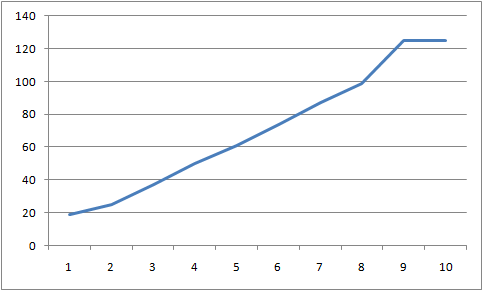
\includegraphics[scale=0.5]{img/io}
\end{center}
\caption{QEMU-KVM Scalability - IO overhead}
\label{fig1}
\end{figure}
\begin{figure}[ht]
\begin{center}
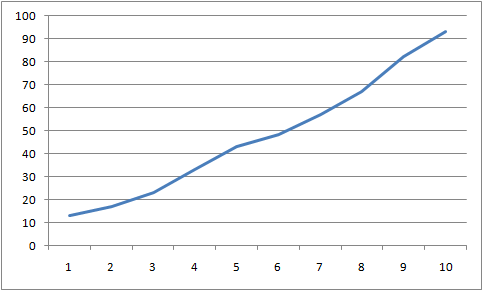
\includegraphics[scale=0.5]{img/cpu}
\end{center}
\caption{QEMU-KVM Scalability - CPU overhead}
\label{fig2}
\end{figure}
\begin{figure}[ht]
\begin{center}
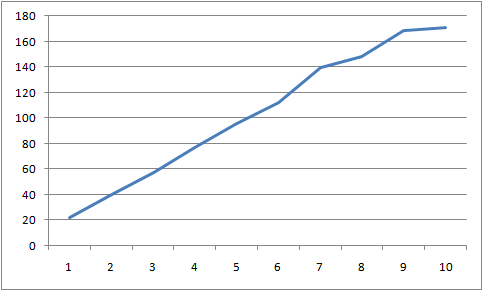
\includegraphics[scale=0.5]{img/net}
\end{center}
\caption{QEMU-KVM Scalability - Network overhead}
\label{fig3}
\end{figure}


\subsection{Experiment conclusions}

Although a central virtual machine server would be more efficient from
an administration and deployment point of view, the costs outweigh the
benefits. Neither the open source KVM solution nor the enterprise VMware
vSphere solution could provide enough virtual machines instances per
physical machine in order to scale.

A single server powerful enough to host 20+ machines is too expensive
compared to other approaches. A cluster of cheaper workstations would be
more cost effective, but still not scale to the required number of
virtual machines needed.

The model was discarded after one semester.


\section{Replacing freezing with LiveCDs}


Freezing of the operating system system is commonly found with LiveCD
(LiveDVD, LiveUSB) Linux distributions. So another idea was to use
LiveCDs instead of a distribution installed on the local hard drive.

But using actual CDs or DVDs was not a good proposal for several
reasons. First, not all workstations have CD/DVD drives and using
\ac{USB} sticks is expensive. Moreover, booting from such device takes
longed than from the hard disk.

Booting LiveCD ISO images off the network using \ac{PXE} would be an
alternative, but, as discussed in previous chapter, PXE has its
drawbacks.

An new idea related to Live distribution booting came along with version
2 of \ac{GRUB}. Grub2 is the next generation Linux bootloader that is
trying to replace the “Legacy” Grub version. It is a complete rewrite of
Grub 1 and only lately becoming fully featured compared to the old
version and even comes with some new interesting features.


An useful new feature in Grub2 is the possibility to boot from an ISO
file. A LiveCD can be stored in an .iso file on disk and loaded by
Grub without having to burn it onto CD or having to boot the normal
system first. A menu entry for ISO booting would look like this:


\begin{verbatim}
menuentry "Ubuntu LiveCD" {
        loopback loop (hd0,1)/boot/iso/ubuntu-12.04-desktop-i386.iso
        linux (loop)/casper/vmlinuz boot=casper
:iso-scan/filename=/boot/iso/ubuntu-12.04-desktop-i386.iso noprompt
noeject
        initrd (loop)/casper/initrd.lz
}
\end{verbatim}

What this feature provides is the possibility of providing a contained
environment (similarly to a friezed system) but stored on the hard disk.
Students could transparently boot the distribution without knowing it's
actually a LiveCD.

If virtual machines or virtual containers are required, they could be
bundled up in a custom Live image packet in a new iso file.

\section{Syncing over the network}

The previous idea, with booting live distributions from iso files on the
disk does replace the need for system freezing, but still needs a
deployment mechanism.

Using UDPcast to copy the disk images to all the stations would also
copy the iso images on the disk. But since now the operating system is
packet inside a single (iso) file rather than on a partition or an
entire disk, we could use other network transfer protocols to copy
files.

\emph{SAMBA} is a good protocol that allows file sharing on the
\ac{LAN}. Better protocols for the given situation is \emph{rsync} or
\emph{\ac{NFS}}. The later two provide a synchronization mechanism
between two sources.


\section{Using Intel vPro technology}


Starting with the its Core 2 processors series, Intel introduced the
\emph{vPro technology}. vPro is an umbrella term for a series of
hardware technologies built into computer chips produced by Intel, among
which, \emph{Intel’s Active Management Technology (AMT)}. The \ac{AMT}
technology allows remote management features to computers that use vPro
processors in order to monitor, maintain, and manage the target computer
regardless of the Operating System (or regardless of the existence of an
Operating System) or its power state. \ac{AMT} and vPro also introduce
security features such as remote shutdown of computers in case of theft.

A description of vPro is available in Whitepaper \cite{paper:intel-vpro}
released by Intel corporation, cited here.

Desktop PCs with Intel® vPro™ technology provide built-in, professional-
grade management and security capabilities that meet critical business
challenges. IT can lower maintenance costs while ensuring greater levels
of IT compliance using Intel vPro technology’s improved remote
management, provisioning, problem resolution, off-hours maintenance, and
proactive security capabilities—all directly from the IT console.

Most importantly, these hardware-based capabilities are available to
authorized IT down-the-wire, even for PCs that are powered off or whose
operating system (OS) is down. IT will now be able to remotely take
accurate asset and hardware/software inventories, contain more security
threats, resolve software and hardware problems faster, and increase
user uptime.

PCs with Intel vPro technology also include additional,
hardware-based capabilities that give IT the option of a lighter-weight
form of virtualization for mainstream business. IT can now run critical
security applications in a simplified, self-contained, dedicated virtual
partition—or “virtual appliance” even while users are working on their
own compute-intensive tasks in the user OS.

These powerful new hardware-based capabilities are designed right into
PCs with Intel vPro technology. And, every PC with Intel vPro technology
uses the Intel® Core™2 Duo processor. The Intel Core 2 Duo processor
gives IT the dual-core, 64-bit capable performance needed to run the
latest compute-intensive applications and provide outstanding user
responsive ness in multitasking environments—all in a power-efficient
design that is Windows Vista* Premium Ready. IT can now spend less time
on routine tasks, and can focus resources where they are most needed for
better manageability and security of desktop PCs.

\subsection{Remote node management}

The \ac{AMT} technology allows for active discovery of the workstations
in the network and then access that workstation using \ac{VNC}. Because
of the built in TCP/IP stack, the workstation will have IP connectivity
even if there is no operating system available.

The control is made via the open standard \ac{VNC} so this means that I
can be controlled by any client running this protocol.

\begin{figure}[ht]
\begin{center}
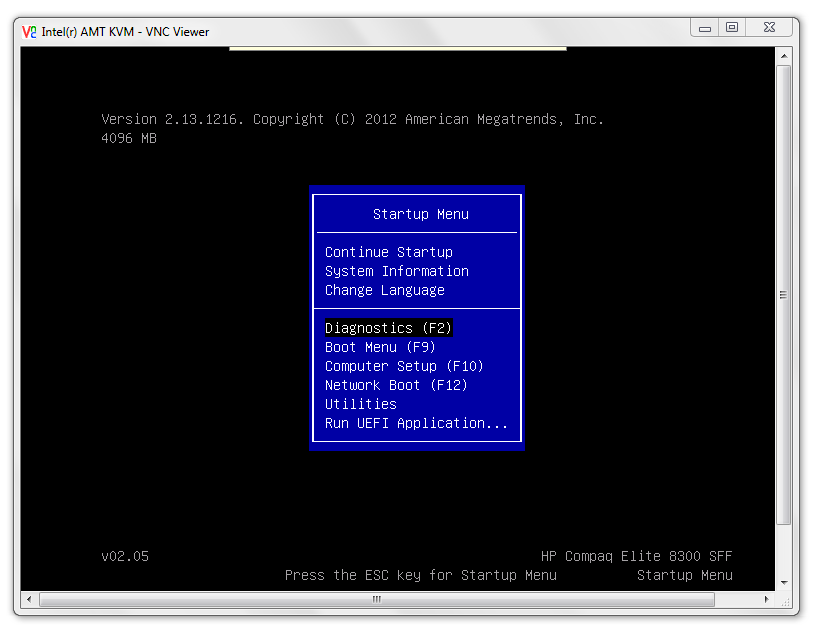
\includegraphics[scale=0.5]{img/intel_amt_bios}
\end{center}
\caption{Accessing BIOS on remote workstation with Intel AMT}
\label{fig1}
\end{figure}


\subsection{Remote ISO boot}


A more relevant feature for the purpose of this thesis is the
\emph{Remote ISO Launcher}. Intel releases a proof-of-concept software
that uses the \ac{AMT} framework, under open source licence. The Remote
ISO Launcher can connect to a remote workstation and transfer via the
network connection an iso image and make the workstation boot the Live
from the network.

This is similar to what \ac{PXE} could do, but \ac{AMT} uses a push,
rather than a pull model. In PXE, the client workstation would as a
\ac{TFTP} server for an image  and boot from it, starting with the
kernel. In AMT, a central station, running the Remote ISO Launcher will
control the remote node, restart it, push the image to it and the client
node would boot. In the second case, at no time would the administer
need to be in front of the client workstation.

At the time of writing this thesis, the version of Remote ISO Launcher
offers just basic operations (like rebooting the remote machine and
booting the ISO). But the API of AMT offers a larger number of
operations (for example, the ability to run commands on the remote
operating system after boot time).

Being open source, the Remote ISO Launcher could be extended to offer
features like sending reboot commands periodically to restart the
operating system, shut down the target computer in off-hours or
scheduling certain images to be load at wanted hours.



% vim: set tw=78 sts=2 sw=2 ts=8 aw et ai:

\chapter{Future available features}\label{ch:future}
\bigskip

The ability of deploying with ease of operating system images on
available workstations brings the possibility of reusing hardware that
in other situations would be unused. This could bring a cost efficient
way of using current hardware.

In a normal research university, you have clusters of servers installed
with the purpose of running computational tasks. These are used whenever
a project needs processing and storage power. Among many projects
running on UPB servers, is VMchecker.

\section{VMchecker}

\emph{VMchecker} is an open sources project started by a group of
teachers and students from the Computer Science Department at the
Politehnica University of Bucharest. The goal was to automate testing of
homework from the Operating Systems and Compilers courses. Since then,
it was been adopted by several other courses, that had assessments
ranging from high level programming, to network simulations to kernel
programming.

The architecture of VMchecker is very modular and uses several
technologies. The infrastructure is organized in three components:
\begin{itemize}
\item vmchecker-ui
\item vmchecker-storer
\item vmchecker-tester
\end{itemize}

The \emph{User Interface} is a web interfaces based on Google Web Toolkit,
a framework with a Java backend and a JavaScript frontend. The UI is used
by students to upload theit assessments, view the results of the automated
tests and view their final grade and feedback.

Assessments uploaded via the web UI, are stored in the repository, on the
\emph{Storer}. Each homework is archived in a Git repository. A student can
submit several revisions of the same assessment, each is tested, but only
the last one (current one) is displayed in the UI. The Storer manages a
queue of assessments that will be send out for checking. This component is
a collection of scripts written in Python or Bash and require 3rd party
modules like PyVix, an API for managing VMware virtual machines. Also on
the Storer, the tests for each homework are stored.

The submitted assessments from the queue on the Storer are passed to the
\emph{Tester}. The Tester has one or more virtual machines (VMware in the
current implementation) that can be started. After a fresh machine is
started, the generic homework tests are uploaded to the virtual machine,
then the submitted assessment. Both the tests and the submitted assessment
is compiled and the test is ran. The output of the tests is saved, along
with other system logs (like kernel logs in dmesg). The results are passed
back to the Stored, from where the UI can hand the results to the students.

\section{Distributing VMchecker tester nodes}

The main bottleneck of the infrastructure is the Tester. The current
implementation of the Tester makes it possible for only one  VMware virtual
machine to be used at one time. This means that all submissions to be
tested need to wait in the same queue. Along with the First Come First
Serve policy, means that submissions at the back of the queue get processed
very slow.

The problem is similar to the one that network traffic faces. Internet
packets are different, some are big, some are small, some are processed
fast, some are processed slow. The default way that packets are routed is
on a First Come First Serve bases, which means that some packets get
treated worse than others. Without a Quality of Services implemented,
theres is no prediction of the treatment of important or unimportant
packets.

From data analysed, current instance of VMchecker has three types of
homework tests:
\begin{itemize}
\item simple tests that run only in userspace an require basic containment
of the test process
\item system or kernel level tests that require root access to the entire
virtual machine
\item full system tests that need the entire virtual machine to be taken as
input
\end{itemize}

The first step of optimising VMchecker is to mark these types of
assessments by the above categories. This means that the Tester will know
what is the estimated time of the testing and can be able to choose smaller
tests in front of bigger tests. If two simple tests that take tens of
seconds are submitted after a test that needs the entire virtual machine to
be copied, all of these will take a matter of minutes in average to get the
result. But if a QoS is implemented, the Tester can choose to run the
smaller tests first, even though the larger test was submitted first.

But as long as the tester can only run a single virtual machine, the queue
can still become long enough to provide bad result times. The obvious
solution is to run multiple virtual machines at the same time so that
several tests can be run simultaneously. But this require adequate hardware
resources.

Running more than one virtual machine on the Tester offers another
optimisation: provisioning machines. In the current implementation every
time a submission is made, the tester start the correct virtual machine for
that test. This takes time because the machine needs to be started or
resumed from a snapshot on the spot. Provisioning machines means that fresh
virtual machines are already started and ready to receive tests to be ran.
In the best case scenario, anytime a test needs to run, a machine is up and
running and is instantly ready to run the test. The machine is cleanup
(closed) after the test is done, but this won't affect the next test,
because that next test will run on another provisioned machine.

But the idea of provisioning brings another question: how many machines to
keep running and of what type? Keeping too many machines running that
aren't needed means that if only one is (or a few are) used, that (or
those) will perform bad because they need to share resources with the other
that are idle.

The proposed algorithm is based on all the optimisations mentioned above.
First of all, the types of virtual machines should vary. Simple tests can
be run on OpenVZ or LXC, rather than VMware full virtualization. The full
system tests could be run on other full virtualization or
paravirtualization like VirtualBox or Xen. Depending on the tests, the
appropriate machine should be used, because an OpenVZ machine is easier to
start and clean compared to a VMware machine, and if a test doesn't need
more than userspace access, resources shouldn't be wasted on it.

Machines should be already started before tests are submitted, meaning that
multiple machines need to be started at the same time. What machines should
be provisioned need to be chosen using an heuristic that takes under
consideration the deadlines of assignments and the live requests made by
the users. If in one day, the number of VMware machines are higher than
usual, OpenVZ machines could be stopped to reallocate resources to the
needed ones.

A related thesis \cite{paper:vmchecker} details the idea of distributing
the Tester infrastructure over several nodes and also the idea of using
several virtualization solutions to increase testing speed.


\section{Using workstations as VMchecker nodes}

Workstations from computer laboratories are mostly used during daytime
for the students to do their tasks. The reset of the time the are
usually shut down. The processing power of those stations could be
harnessed during the off work hours.

As seen earlier, using vPro \ac{AMT}, booting a live distribution on the
network is an easy task. The VMchecker server could command the
laboratory workstations to boot up a special vmchecker image that
contains the Tester component. This way, VMchecker could have access to
tens of Testers that would greatly improve the efficiency  of the
automated grading system.

% vim: set tw=78 sts=2 sw=2 ts=8 aw et ai:

\chapter{Conclustions}\label{ch:conclusions}
\bigskip


The previous chapters discussed many technologies and
protocols that each provided needed features. But an efficient
management procedure would make use of a combination of all of them.
The following are some recommended procedures that resulted from the
research and experimenting done.

First of all, the old freezing system should be phased out. Because of
its lack of current development it has become inefficient for the
present needs. The "clean environment" features could be replaced by
running Live Linux distributions and using virtual machines.

Image multiplication actions that take place at least once per semester
or at every course beginning should be heavily reduced. Every
workstation should be imaged with a standard operating system that could
self update itself.

The standard operating system should be ready do use virtualization
software, like \ac{KVM} to run virtual systems if needed. It should also
have a pool of Live distribution iso files available for Grub2. The iso
as well as the virtual machines should be kept up to date by
synchronizing over the network with protocols such as \ac{NFS} or rsync.

In case a machine is malfunctioning, it could be remotely accessed using
vPro AMT and fixed remotely.

As we saw, using the approaches presented, projects can benefit from new
features, like VMchecker. Having a cluster or workstations that could be
used non stop and having a easy to use administration system to
provision resources and push new operating system images towards them in
order to accomplish a desired task, could greatly increase the efficiency
of hardware utilization and lowering costs processing power.


\section{Future work}

Being the newest technology presented, Intel's vPro AMT is a framework
where new research could be done. Because it is new, there is a lack of
software that exploits its features. But because it is a feature-full
framework many new ideas could be built on top.

As discussed previously, a scheduling system that would push images
automatically to workstations following timetables in a database could
reduce some manual tasks being done by an administrator that wants to
provision a pool of systems. Such a software project doesn't exist at
the time of writing this thesis and could be a starting point for a new
project.

The idea of a self-updating system has been discussed in this paper, in
order to make workstations automatically use the latest versions of
system images (either Live systems or virtual machines). Going further,
a self-repairing system could take one more set towards eliminating jobs
that an administrator would do. In a distributed self-repairing system,
one node could verify is another is malfunctioning and use its own
system to mirror the other node.

As the VMchecker case study has shown, there are some types of projects
that would benefit from a model where services could benefit on-the-fly
from workstations that aren't used for something else. Searching for
other case studies could prove to be important research.


%\addtocontents{toc}{\protect\clearpage} % <--- just debug stuff, ignore
%\include{multiToC} % <--- just debug stuff, ignore for your documents
% ********************************************************************
% Backmatter
%*******************************************************
\appendix
\cleardoublepage%\part{Appendix}
%\include{chapters/Chapter0A}
%********************************************************************
% Other Stuff in the Back
%*******************************************************
\cleardoublepage%********************************************************************
% Bibliography
%*******************************************************
% work-around to have small caps also here in the headline
\manualmark
\markboth{\spacedlowsmallcaps{\bibname}}{\spacedlowsmallcaps{\bibname}} % work-around to have small caps also
%\phantomsection 
\refstepcounter{dummy}
\addtocontents{toc}{\protect\vspace{\beforebibskip}} % to have the bib a bit from the rest in the toc
\addcontentsline{toc}{chapter}{\tocEntry{\bibname}}
\bibliographystyle{plainnat}
\label{app:bibliography}
\bibliography{bibliography}

%\cleardoublepage\pagestyle{empty}

\hfill

\vfill


\pdfbookmark[0]{Colophon}{colophon}
\section*{Colophon}
This thesis was typeset with \LaTeXe\ using Hermann Zapf's
\emph{Palatino}
and \emph{Euler} type faces (Type~1 PostScript fonts \emph{URW
Palladio L}
and \emph{FPL} were used). The listings are typeset in \emph{Bera
Mono}, originally developed by Bitstream, Inc. as ``Bitstream Vera''.
(Type~1 PostScript fonts were made available by Malte Rosenau and
Ulrich Dirr.)

The typographic style was inspired by \cauthor{bringhurst:2002}'s genius as
presented in \emph{The Elements of Typographic Style} 
\citep{bringhurst:2002}. It is available for \LaTeX\ via \textsmaller{CTAN} as 
``\href{http://www.ctan.org/tex-archive/macros/latex/contrib/classicthesis/}%
{\texttt{classicthesis}}''.

\paragraph{note:} The custom size of the textblock was calculated
using the directions given by Mr. Bringhurst (pages 26--29 and
175/176). 10~pt Palatino needs  133.21~pt for the string
``abcdefghijklmnopqrstuvwxyz''. This yields a good line length between
24--26~pc (288--312~pt). Using a ``\emph{double square textblock}''
with a 1:2 ratio this results in a textblock of 312:624~pt (which
includes the headline in this design). A good alternative would be the
``\emph{golden section textblock}'' with a ratio of 1:1.62, here
312:505.44~pt. For comparison, \texttt{DIV9} of the \texttt{typearea}
package results in a line length of 389~pt (32.4~pc), which is by far
too long. However, this information will only be of interest for
hardcore pseudo-typographers like me.%

To make your own calculations, use the following commands and look up
the corresponding lengths in the book:
\begin{verbatim}
    \settowidth{\abcd}{abcdefghijklmnopqrstuvwxyz}
    \the\abcd\ % prints the value of the length
\end{verbatim}
Please see the file \texttt{classicthesis.sty} for some precalculated 
values for Palatino and Minion.

    \settowidth{\abcd}{abcdefghijklmnopqrstuvwxyz}
    \the\abcd\ % prints the value of the length


\bigskip

\noindent\finalVersionString




%\cleardoublepage%*******************************************************
% Declaration
%*******************************************************
\refstepcounter{dummy}
\pdfbookmark[0]{Declaration}{declaration}
\chapter*{Declaration}
\thispagestyle{empty}
Put your declaration here.
\bigskip
 
\noindent\textit{\myLocation, \myTime}

\smallskip

\begin{flushright}
    \begin{tabular}{m{5cm}}
        \\ \hline
        \centering\myName \\
    \end{tabular}
\end{flushright}

% ********************************************************************
% Game Over: Restart, Restore or Quit?
%*******************************************************
\end{document}
% ********************************************************************
